\begin{table*}[t]
\centering\small
\begin{tabular}{p{0.31\textwidth}rrrr}
\toprule
Branch & Documents & Measured duration & Receipt words & Common tokens\\
\midrule
Publisher audio / unverified ASR & 20 & 22.69 h & 226,093 & 226,138\\
Authored / publisher text & 16 & not comparable & 13,575 & 13,556\\
\bottomrule
\end{tabular}
\caption{Actual analysis branches. Receipt words have different source-specific definitions and must not be pooled as a common denominator. Audio has nineteen Bashar-related source contexts and one Ashtar-attributed creator episode; written material has fifteen Daniel items and one Paul transcript.}
\label{tab:corpus}
\end{table*}
\begin{figure*}[t]
\centering
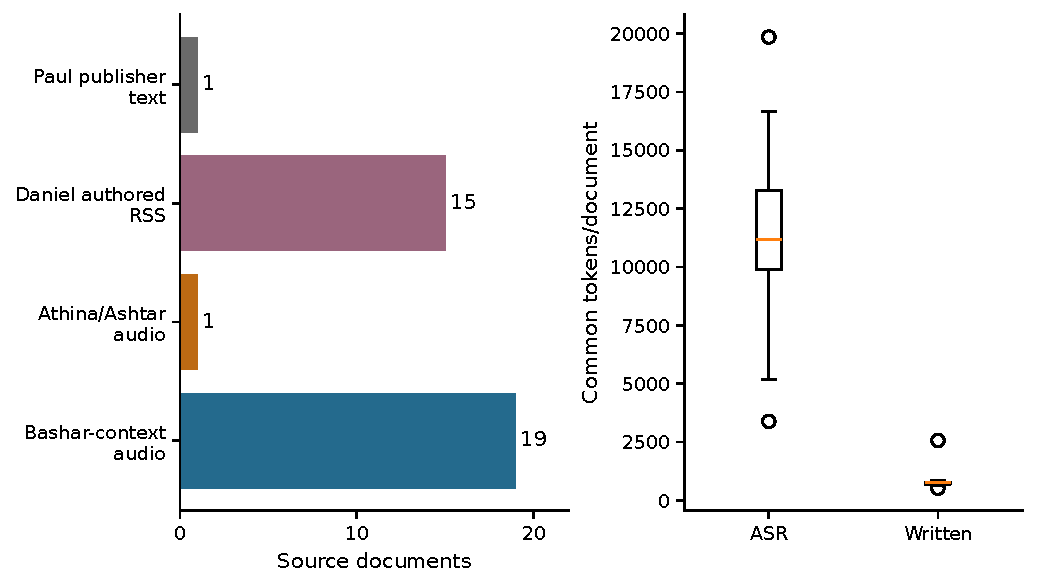
\includegraphics[width=\textwidth]{generated/figures/source-coverage.pdf}
\caption{Thirty-six source documents are two distinct modalities. Nineteen of 20 audio recordings have Bashar context; the one Ashtar-attributed creator episode is a singleton. This is not a balanced sample of mediums or civilizations. Token counts use the common analytical tokenizer, not acquisition receipt word definitions.}
\label{fig:source-coverage}
\end{figure*}
